\section{Lecture 14: 24.09.2025}

\subsection{Convergence}
Let $A = X \Lambda X^{-1}$, $\Lambda = \mathrm{diag}(\lambda_1, \ldots, \lambda_n)$ and $\kappa_2(A) = \|A\|_2 \|A^{-1}\|_2 = \frac{\lambda_{\max}}{\lambda_{\min}}$ if $A$ is \emph{SPD}.

\begin{itemize}
    \item \textbf{CG:}
          \[
              \|\mathbf{x}_\star - \mathbf{x}_m\|_A \leq 2\left(\frac{\sqrt{\kappa_2(A)} - 1}{\sqrt{\kappa_2(A)} + 1}\right)^m \|\mathbf{x}_\star - \mathbf{x}_0\|_A
          \]
    \item \textbf{GMRES:} $\lambda(A) \subset \mathrm{E}(c,d,a)$: The set of eigenvalues is enclosed in an ellipse with center $c$, focal distance $d$ and semi-major axis $a$. Then:
          \[
              \|\mathbf{r}_m\|_2 \le \|X\|_2\|X^{-1}\|_2
              \min_{\substack{p\in\mathbb{P}_m\\p(0)=1}}
              \max_{z\in \mathrm{E}(c,d,a)} |p(z)| \;\|\mathbf{r}_0\|_2.
          \]
          For an ellipse one can use Chebyshev-type estimates to get an explicit geometric rate. Defining
          \[
              q \coloneqq \frac{a-\sqrt{a^2-d^2}}{a+\sqrt{a^2-d^2}}\quad(0<q<1),
          \]
          one convenient bound is
          \[
              \|\mathbf{r}_m\|_2 \le 2\,\|X\|_2\|X^{-1}\|_2\, q^{\,m}\,\|\mathbf{r}_0\|_2,
          \]
          where the factor 2 depends on the normalization of the minimax polynomial and can be omitted in some formulations.

          \begin{center}
              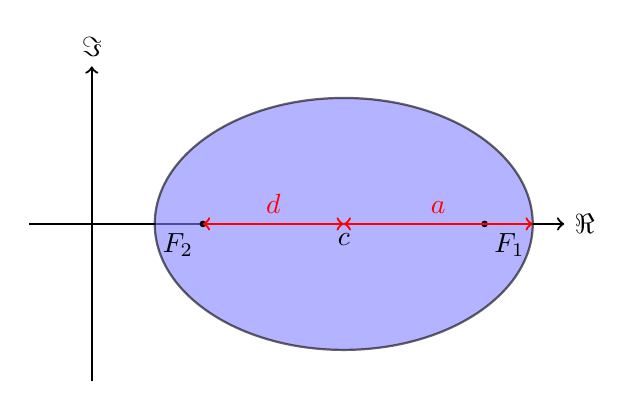
\begin{tikzpicture}[scale=0.8]
                  \pgfmathsetmacro{\a}{3}   % semi-major
                  \pgfmathsetmacro{\b}{2}   % semi-minor
                  \pgfmathsetmacro{\f}{sqrt(\a*\a-\b*\b)} % focal distance = d
                  \coordinate (C) at (4,0);
                  % axes
                  \draw[->,thick] (-1,0) -- (7.5,0) node[right] {$\Re$};
                  \draw[->,thick] (0,-2.5) -- (0,2.5) node[above] {$\Im$};
                  % ellipse
                  \draw[thick,fill=blue!50,draw=black,opacity=0.6] (C) ellipse (\a cm and \b cm);
                  % center and foci
                  \node[below] at (C) {$c$};
                  \fill (4+\f,0) circle (1.5pt) node[below right] {$F_1$};
                  \fill (4-\f,0) circle (1.5pt) node[below left] {$F_2$};
                  % labels for a and d
                  \draw[<->,thick, red] (C) -- ++(\a,0) node[midway, above] {$a$};
                  \draw[<->,thick, red] (C) -- ++(-\f,0) node[midway, above] {$d$};
              \end{tikzpicture}
          \end{center}
\end{itemize}

\subsection{Preconditioning (Saad, Chap. 9)}

\[
    A\mathbf{x} = \mathbf{b}
\]

Rewrite the system by choosing $M \in \mathbb{R}^{n \times n}$.

\begin{itemize}
    \item \textbf{Left preconditioning (LPC):} $M^{-1} A \mathbf{x} = M^{-1} \mathbf{b}$, solve for $\mathbf{x}$.
    \item \textbf{Right preconditioning (RPC):} $A M^{-1} \mathbf{u} = \mathbf{b}$, solve for $\mathbf{u} = M \mathbf{x}$ or $\mathbf{x} = M^{-1} \mathbf{u}$.
          \[
              \tilde{A} = A M^{-1}
          \]
\end{itemize}

Apply \textbf{RPC} for $A$, $\mathbf{b}$ and $\mathbf{x}_0$ where:
\[
    \mathbf{u}_0 = M \mathbf{x}_0, \quad \mathbf{r}_0 = \mathbf{b} - A \mathbf{x}_0 = \mathbf{b} - A M^{-1} \mathbf{u}_0 = \mathbf{b} - A M^{-1}M \mathbf{x}_0
\]
Start with the \emph{Arnoldi process} with right preconditioning:
\begin{algorithm}[H]
    \caption{Arnoldi process with RPC}
    \label{alg:arnoldi_rpc}
    \begin{algorithmic}
        \State $\beta = \|\mathbf{r}_0\|_2$, $\mathbf{v}_1 = \mathbf{r}_0 / \beta$
        \State $\mathbf{w}_j = A M^{-1} \mathbf{v}_j$
        \For{$i = 1, 2, \ldots, j$}
        \State $h_{ij} = \langle \mathbf{w}_j, \mathbf{v}_i \rangle$
        \State $\mathbf{w}_j = \mathbf{w}_j - h_{ij} \mathbf{v}_i$
        \EndFor
        \State $h_{j+1,j} = \|\mathbf{w}_j\|_2$
        \If{$h_{j+1,j} = 0$}
        \State Stop
        \EndIf
        \State $\mathbf{v}_{j+1} = \mathbf{w}_j / h_{j+1,j}$
        \Return $\overline{H}_m, V_m$
    \end{algorithmic}
\end{algorithm}

Now we solve for:
\begin{align*}
    \overline{H}_m \mathbf{y}_m & = \beta \mathbf{e}_1 \tag{Least squares problem}                                         \\
    \mathbf{u}_m                & = \mathbf{u}_0 + V_m \mathbf{y}_m                                                        \\
    \mathbf{x}_m                & = M^{-1} \mathbf{u}_0 + M^{-1} V_m \mathbf{y}_m = \mathbf{x}_0 + M^{-1} V_m \mathbf{y}_m
\end{align*}
So $\mathbf{u}_m$ is never computed explicitly, we only need to compute:
\[
    M^{-1} \mathbf{v}_j = \mathbf{z}_j \quad \Rightarrow \quad M \mathbf{z}_j = \mathbf{v}_j
\]
This has to be solved for each iteration (and store $\mathbf{z}_j$ instead of $\mathbf{v}_j$).

For the \textbf{LPC} we have:
\[
    \mathbf{r}_j = M^{-1} (\mathbf{b} - A \mathbf{x}_j)
\]


\subsection{Conjugate Gradient}
$A$ is \emph{SPD} and $\tilde{A} = M^{-1} A$ is \emph{SPD}, choose $M = L L^T$ SPD (Cholesky factorization).
\begin{align*}
    M                                         & = L L^T                                                                                                                                          \\
    M^{-1}                                    & = L^{-T} L^{-1}                                                                                                                                  \\
    M^{-1} A \mathbf{x}                       & = M^{-1} \mathbf{b}                                                                                                                              \\
    (L^{-T} L^{-1}) A I \mathbf{x}            & = L^{-T} L^{-1} \mathbf{b}                                                                                                                       \\
    (L^{-T} L^{-1}) A (L^{-T} L^T) \mathbf{x} & = L^{-T} L^{-1} \mathbf{b}                                                                                                                       \\
    L^{-T} (L^{-1} A L^{-T}) (L^T \mathbf{x}) & = L^{-T} (L^{-1} \mathbf{b})                                                                                                                     \\
    (L^{-1} A L^{-T}) (L^T \mathbf{x})        & = L^{-1} \mathbf{b}                                                                                                                              \\
    \tilde{A} \tilde{\mathbf{x}}              & = \tilde{\mathbf{b}} \quad \text{with } \tilde{A} = L^{-1} A L^{-T}, \tilde{\mathbf{x}} = L^T \mathbf{x}, \tilde{\mathbf{b}} = L^{-1} \mathbf{b}
\end{align*}


\begin{algorithm}[ht]
    \caption{Preconditioned Conjugate Gradient (PCG) on $\tilde{A}\tilde{\mathbf{x}}=\tilde{\mathbf{b}}$}
    \label{alg:pcg_tilde}
    \begin{algorithmic}
        \State Choose initial guess $\tilde{\mathbf{x}}_0$ (e.g.\ $\tilde{\mathbf{x}}_0 = L^T \mathbf{x}_0$)
        \State $\tilde{\mathbf{r}}_0 = \tilde{\mathbf{b}} - \tilde{A}\tilde{\mathbf{x}}_0$
        \State $\tilde{\mathbf{p}}_0 = \tilde{\mathbf{r}}_0$
        \For{$j= 0,1,2,\ldots$}
        \State $\alpha_j= \dfrac{\langle \tilde{\mathbf{r}}_j, \tilde{\mathbf{r}}_j\rangle}{\langle \tilde{A}\tilde{\mathbf{p}}_j, \tilde{\mathbf{p}}_j\rangle}$
        \State $\tilde{\mathbf{x}}_{j+1} = \tilde{\mathbf{x}}_j+ \alpha_j\tilde{\mathbf{p}}_j$
        \State $\tilde{\mathbf{r}}_{j+1} = \tilde{\mathbf{r}}_j- \alpha_j\tilde{A}\tilde{\mathbf{p}}_j$
        \If{$\|\tilde{\mathbf{r}}_{j+1}\|_2 < \text{tol}$}
        \State Stop
        \EndIf
        \State $\beta_j= \dfrac{\langle \tilde{\mathbf{r}}_{j+1}, \tilde{\mathbf{r}}_{j+1} \rangle}{\langle \tilde{\mathbf{r}}_j, \tilde{\mathbf{r}}_j\rangle}$
        \State $\tilde{\mathbf{p}}_{j+1} = \tilde{\mathbf{r}}_{j+1} + \beta_j\tilde{\mathbf{p}}_j$
        \EndFor
        \State Return $\tilde{\mathbf{x}}_m$ and transform back $\mathbf{x}_m = L^{-T}\tilde{\mathbf{x}}_m$
    \end{algorithmic}
\end{algorithm}

We see that the inner products in $\alpha_j$ and $\beta_j$ can be rewritten:
\begin{align*}
    \langle \tilde{\mathbf{r}}_j, \tilde{\mathbf{r}}_j \rangle           & = \tilde{\mathbf{r}}_j^T \tilde{\mathbf{r}}_j                                \\
                                                                         & = \langle L^{-1} \mathbf{r}_j, L^{-1} \mathbf{r}_j \rangle                   \\
                                                                         & = \langle \mathbf{r}_j, L^{-T} L^{-1} \mathbf{r}_j \rangle                   \\
                                                                         & = \langle \mathbf{r}_j, M^{-1} \mathbf{r}_j \rangle                          \\
                                                                         & = \|\mathbf{r}_j\|_M^2                                                       \\
    \langle \tilde{A} \tilde{\mathbf{p}}_j, \tilde{\mathbf{p}}_j \rangle & = \langle L^{-1} A L^{-T} \tilde{\mathbf{p}}_j, \tilde{\mathbf{p}}_j \rangle \\
                                                                         & = \langle L^{-1} A \mathbf{p}_j, \tilde{\mathbf{p}}_j \rangle                \\
                                                                         & = \langle A \mathbf{p}_j, L^{-T} \tilde{\mathbf{p}}_j \rangle                \\
                                                                         & = \langle A \mathbf{p}_j, \mathbf{p}_j \rangle
\end{align*}

Then the iterations become:
\begin{align*}
    \mathbf{x}_{j+1} & = \mathbf{x}_j + \alpha_j L^{-T} L^T \mathbf{p}_j = \mathbf{x}_j + \alpha_j \mathbf{p}_j                                      \\
    \mathbf{r}_{j+1} & = \mathbf{r}_j - \alpha_j \overbrace{L L^{-1} A L^{-T} L^T}^{\tilde{A}} \mathbf{p}_j = \mathbf{r}_j - \alpha_j A \mathbf{p}_j \\
    \mathbf{p}_{j+1} & = L^{-T} L^{-1} \mathbf{r}_{j+1} + \beta_j \mathbf{p}_j = M^{-1} \mathbf{r}_{j+1} + \beta_j \mathbf{p}_j
\end{align*}

Then we have the \textbf{Preconditioned Conjugate Gradient (PCG) algorithm}:
\begin{algorithm}[H]
    \caption{Preconditioned Conjugate Gradient (PCG)}
    \begin{algorithmic}
        \State $\mathbf{r}_0 = \mathbf{b} - A \mathbf{x}_0$, $\mathbf{z}_0 = M^{-1} \mathbf{r}_0$, $\mathbf{p}_0 = \mathbf{z}_0$
        \For{$j = 0,1,2,\ldots$}
        \State $\alpha_j = \dfrac{\langle \mathbf{r}_j, \mathbf{z}_j \rangle}{\langle A \mathbf{p}_j, \mathbf{p}_j \rangle}$
        \State $\mathbf{x}_{j+1} = \mathbf{x}_j + \alpha_j \mathbf{p}_j$
        \State $\mathbf{r}_{j+1} = \mathbf{r}_j - \alpha_j A \mathbf{p}_j$
        \If{$\|\mathbf{r}_{j+1}\|_2 < \text{tol}$}
        \State Stop
        \EndIf
        \State $\mathbf{z}_{j+1} = M^{-1} \mathbf{r}_{j+1}$
        \State $\beta_j = \dfrac{\langle \mathbf{r}_{j+1}, \mathbf{z}_{j+1} \rangle}{\langle \mathbf{r}_j, \mathbf{z}_j \rangle}$
        \State $\mathbf{p}_{j+1} = \mathbf{z}_{j+1} + \beta_j \mathbf{p}_j$
        \EndFor
        \Return $\mathbf{x}_m$
    \end{algorithmic}
\end{algorithm}

The price we pay for preconditioning with $M$ is that we have to solve a linear system $M \mathbf{z}_j = \mathbf{r}_j$ at each iteration, and store $\mathbf{z}_j$.

\paragraph{How to choose $M$?}
\begin{itemize}
    \item $M$ should be \emph{SPD} if $A$ is \emph{SPD} (when using PCG).
    \item $M$ should be a good approximation of $A$ (in some sense), i.e. $M \approx A$ so that $\kappa(\tilde{A}) < \kappa(A)$.
    \item $M$ should be cheap to apply, i.e.\ solving $M \mathbf{z} = \mathbf{r}$ should be cheap.
    \item $M$ should be sparse (if $A$ is sparse).
    \item if $A$ is \emph{SPD}, then $M$ should also be \emph{SPD}.
\end{itemize}

\paragraph{In this course:}
\begin{enumerate}
    \item Use one iteration of one of the \emph{stationary methods} (e.g. Jacobi, Gauss-Seidel, SOR).
    \begin{itemize}
        \item Jacobi: $M = D$ (diagonal of $A$).
        \item Gauss-Seidel: $M = D + L$ (lower triangular part of $A$).
        \item SOR: $M = \frac{1}{\omega} D + L$.
    \end{itemize}
    \item Incomplete factorizations
            \begin{itemize}
                \item Incomplete LU (ILU) for general $A \approx LU$. LU keeps the sparsity structure of $A$.
                \item Incomplete Cholesky (IC) for \emph{SPD} $A \approx LL^T$.
            \end{itemize}
    \item \emph{Multigrid methods}
\end{enumerate}
